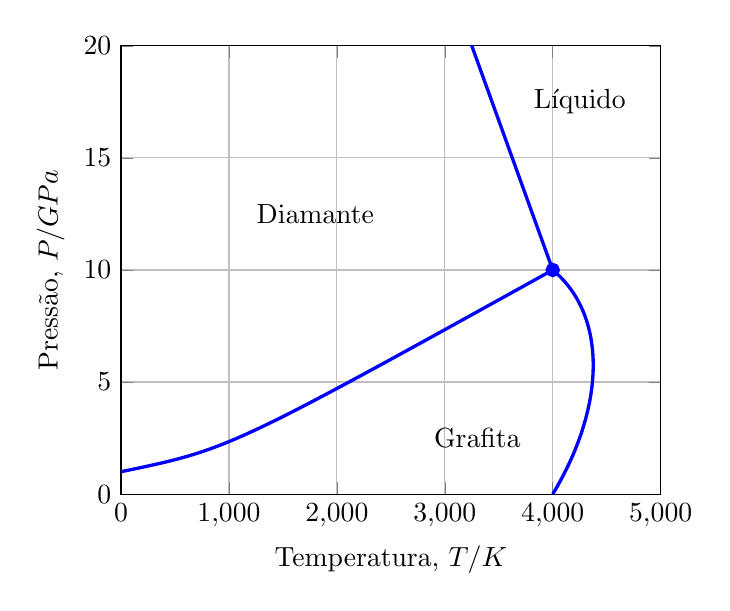
\begin{tikzpicture}
\begin{axis}
    [
        grid = major,
        ylabel = {Pressão, $P/\unit{GPa}$},
        xlabel = {Temperatura, $T/\unit{K}$},
        ymin=0, ymax=20,
        xmin=0, xmax=5000,
    ]       
    \draw [draw=blue, very thick]
        (axis cs: 4000, 10) .. controls (4500, 8) and (4500, 4) .. (axis cs: 4000, 0);
    \draw [draw=blue, very thick]
        (axis cs: 4000, 10) -- (axis cs: 2500, 30);
    \draw [draw=blue, very thick]
        (axis cs: 0, 1) .. controls (1000, 2) .. (axis cs: 4000, 10);

    \addplot [ mark=*, color=blue, very thick ] coordinates
        { 
            (4000, 10) 
        };

    \node [anchor = center] at (axis cs: 4250, 17.5) 
        { Líquido };
    \node [anchor = center] at (axis cs: 3300, 2.5) 
        { Grafita };
    \node [anchor = center] at (axis cs: 1800, 12.5) 
        { Diamante };
\end{axis}
\end{tikzpicture}
    